	\section*{13/09}
	
	\begin{center}
	\textbf{Одномерные пружинные системы}
	\end{center}
	
	 \begin{figure}[h] 
	\begin{center}
	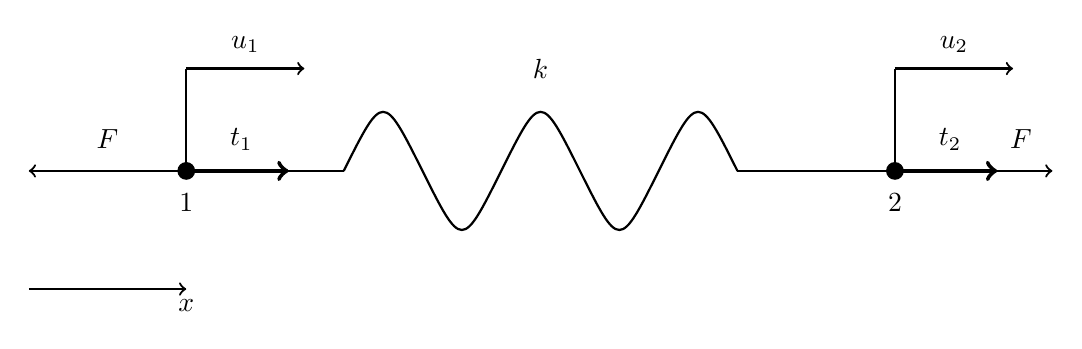
\begin{tikzpicture}
	\draw[thick] (-2, 0) -- (0, 0);
    \draw[thick] (0,0) 

        .. controls +(0.5,1) and +(-0.5,1) .. (1,0)
        .. controls +(0.5,-1) and +(-0.5,-1) .. (2,0)
        .. controls +(0.5,1) and +(-0.5,1) .. (3,0)
        .. controls +(0.5,-1) and +(-0.5,-1) .. (4,0)
        .. controls +(0.5,1) and +(-0.5,1) .. (5,0);
        
       	\node at (2.5, 1.3) {$k$};

    \draw[thick] (5,0);
    \draw[thick] (5, 0) -- (7, 0);
    
    \filldraw (-2, 0) circle (3pt);
     \node  at (-2,-0.4) {1};
    \filldraw (7, 0) circle (3pt);
     \node  at (7,-0.4) {2};
    
    \draw[->][ultra thick] (-2,0) -- (-0.7,0);
    \draw[->][ultra thick] (7,0) -- (8.3,0);
    \node at (-1.3, 0.4) {$t_1$};
    \node at (7.7, 0.4) {$t_2$};
    
    \draw[->][thick] (-2,0) -- (-4,0);
    \draw[->][thick] (7,0) -- (9,0);
     \node at (-3, 0.4) {$F$};
    \node at (8.6, 0.4) {$F$};
    
    \draw[thick] (-2,0) -- (-2,1.3);
    \draw[thick] (7,0) -- (7,1.3);
    \draw[->][thick] (-2,1.3) -- (-0.5,1.3);
    \draw[->][thick] (7,1.3) -- (8.5,1.3);
    \node at (-1.25, 1.6) {$u_1$};
    \node at (7.75, 1.6) {$u_2$};
    
     \draw[->][thick] (-4,-1.5) -- (-2,-1.5) node[below] {$x$};
	\end{tikzpicture}
	\end{center}
	 \caption{Одномерная пружинная система из одного элемента}
 \end{figure}

	
	\textbf{1.} \underline{Уравнение равновесия}
	
	где $k$ - коэффициент жесткости, $u_1, u_2$ - перемещения, $F$ - приложенная сила, $t_1, t_2$ - реакции. 
	
	Закон Гука:
	\[
	F= k\Delta = k(u_2-u_1)
	\]
	\[
	t_1+t_2=0 \rightarrow t_1=-t_2
	\]
	\[
	F=t_2=k(u_2-u_1)
	\]
	\[
	-F=t_1=-k(u_2-u_1)=k(u_1-u_2)
	\]
	\[
	\begin{bmatrix}
		k & - k \\ -k & k
	\end{bmatrix}
	\begin{bmatrix}
	u_1 \\ u_2
	\end{bmatrix} = \begin{bmatrix}
	t_1 \\ t_2
	\end{bmatrix}  \Leftrightarrow Kq=t
	\]
	
	где $q = \begin{bmatrix}
		u_1 \\ u_2
	\end{bmatrix},\ t = \begin{bmatrix}
	t_1 \\ t_2
	\end{bmatrix}, \ K =	\begin{bmatrix}
	k & - k \\ -k & k
	\end{bmatrix}$.\\

\textbf{2.} \underline{Вариационный метод}

\[
\text{П} = \text{П}_{in} - \text{П}_{ex},
\]

где $\text{П}$ - потенциальная энергия системы. 
\[
\text{П}_{in} = \int\limits_0^{\Delta} Fd\Delta = \int\limits_0^{\Delta}k\Delta d\Delta = \frac{k(u_2-u_1)^2}{2}=\frac{1}{2}q^{\text{Т}}Kq=\frac{1}{2}\begin{bmatrix}
		u_1 & u_2
	\end{bmatrix}\begin{bmatrix}
	k & - k \\ -k & k
	\end{bmatrix}
	\begin{bmatrix}
	u_1 \\ u_2
	\end{bmatrix}
\]
\[
\text{П}_{ex} =  t_1 u_1 +t_2 u_2 = q^{\text{Т}}t
\]
\[
\text{П} = \frac{1}{2}q^{\text{Т}}Kq-q^{\text{Т}}t\rightarrow min
\]

Условие стационарности потенциальной энергии
\[
\frac{\partial \text{П}}{\partial q}=0 \Leftrightarrow \frac{\partial \text{П}}{\partial u_1}=0, \ \frac{\partial \text{П}}{\partial u_2}=0
\]
\[
\text{П}=\frac{k}{2}(u_2-u_1)^2-t_1u_1-t_2u_2
\]
\[
\frac{\partial \text{П}}{\partial u_1}=k(u_2-u_1)(-1)-t_1=0 \Leftarrow k(u_1-u_2)= t_1
\]
\[
\frac{\partial \text{П}}{\partial u_2}=k(u_2-u_1)-t_2=0 \Leftarrow k(u_2-u_1)= t_2
\]
\[
\begin{bmatrix}
	k & - k \\ -k & k
\end{bmatrix}
\begin{bmatrix}
	u_1 \\ u_2
\end{bmatrix} = \begin{bmatrix}
	t_1 \\ t_2
\end{bmatrix} 
\]

\textbf{3.} \underline{Метод возможных перемещений}

Работа внутренних сил на возможных деформациях равна внешней работе возможных перемещений:
\[
A_{in}=A_{ex},
\]

где $A_{in}$ - работа внутренних сил на возможных деформациях, 

$A_{ex}$ - работа внешних сил на возможных перемещениях.
\[
A_{in}=F\delta\Delta = F(\delta u_2- \delta u_1)
\]
\[
A_{ex}= t_1\delta u_1 + t_2\delta u_2
\]
\[
F(\delta u_2- \delta u_1)=t_1\delta u_1 + t_2\delta u_2
\]
\[
\delta u_1, \delta u_2 :  \begin{cases}
	- F=t_1 \\ F=t_2
\end{cases}
\]

\textbf{Методика составления глобальной системы для МКЭ}

 \begin{figure}[h]
\begin{center}
	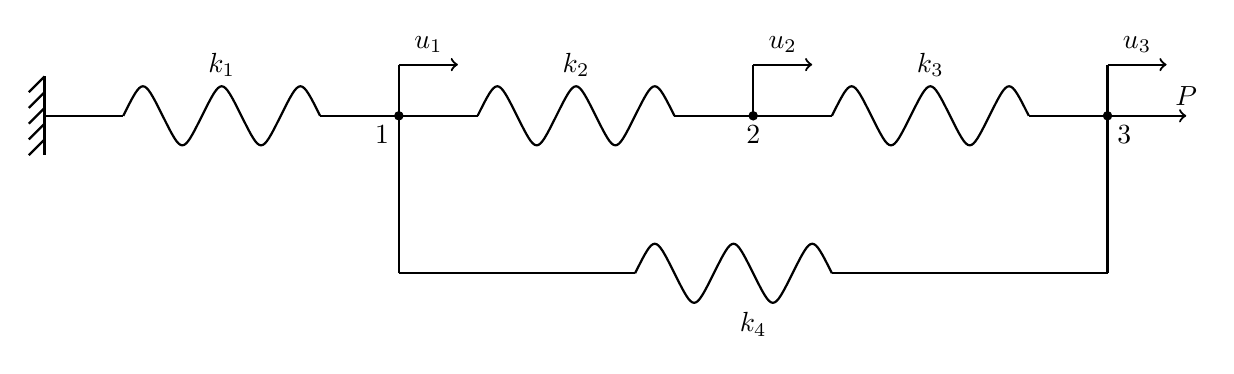
\begin{tikzpicture}[scale=0.5]
	%1 element
	\draw[thick] (-11, 1) -- (-11, -1);
	\draw[thick] (-11.4, 0.6) -- (-11, 1);
	\draw[thick] (-11.4, 0.2) -- (-11, 0.6);
	\draw[thick] (-11.4, -0.2) -- (-11, 0.2);
	\draw[thick] (-11.4, -0.6) -- (-11, -0.2);
	\draw[thick] (-11.4, -1) -- (-11, -0.6);
	
	\draw[thick] (-11, 0) -- (-9, 0);
    \draw[thick] (-9,0) 

        .. controls +(0.5,1) and +(-0.5,1) .. (-8,0)
        .. controls +(0.5,-1) and +(-0.5,-1) .. (-7,0)
        .. controls +(0.5,1) and +(-0.5,1) .. (-6,0)
        .. controls +(0.5,-1) and +(-0.5,-1) .. (-5,0)
        .. controls +(0.5,1) and +(-0.5,1) .. (-4,0);
        
       	\node at (-6.5, 1.3) {$k_1$};
	\draw[thick] (-4, 0);
    	\draw[thick] (-4, 0) -- (-2, 0);
	
	%2 element
	\draw[thick] (-2, 0) -- (0, 0);
    \draw[thick] (0,0) 

        .. controls +(0.5,1) and +(-0.5,1) .. (1,0)
        .. controls +(0.5,-1) and +(-0.5,-1) .. (2,0)
        .. controls +(0.5,1) and +(-0.5,1) .. (3,0)
        .. controls +(0.5,-1) and +(-0.5,-1) .. (4,0)
        .. controls +(0.5,1) and +(-0.5,1) .. (5,0);
        
       	\node at (2.5, 1.3) {$k_2$};

    \draw[thick] (5,0);
    \draw[thick] (5, 0) -- (7, 0);
    
    \filldraw (-2, 0) circle (3pt) node[below left] {1};
    \filldraw (7, 0) circle (3pt) node[below] {2};
    
    \draw[thick] (-2,0) -- (-2,1.3);
    \draw[thick] (7,0) -- (7,1.3);
    \draw[->][thick] (-2,1.3) -- (-0.5,1.3);
    \draw[->][thick] (7,1.3) -- (8.5,1.3);
    \node at (-1.25, 1.8) {$u_1$};
    \node at (7.75, 1.8) {$u_2$};
    
    %3 element
	\draw[thick] (7, 0) -- (9, 0);
    \draw[thick] (9,0) 

        .. controls +(0.5,1) and +(-0.5,1) .. (10,0)
        .. controls +(0.5,-1) and +(-0.5,-1) .. (11,0)
        .. controls +(0.5,1) and +(-0.5,1) .. (12,0)
        .. controls +(0.5,-1) and +(-0.5,-1) .. (13,0)
        .. controls +(0.5,1) and +(-0.5,1) .. (14,0);
        
       	\node at (11.5, 1.3) {$k_3$};
	\draw[thick] (14, 0);
    	\draw[thick][->] (14, 0) -- (18, 0) node[above] {$P$};
	
	\filldraw (16, 0) circle (3pt) node[below right] {3};
	
	 \draw[thick] (16,0) -- (16,1.3);
	 \draw[->][thick] (16,1.3) -- (17.5,1.3);
	 \node at (16.75, 1.8) {$u_3$};
	 
	 %4 element
	 \draw[thick] (-2, -4) -- (-2,0);
	\draw[thick] (-2, -4) -- (4,-4);
    \draw[thick] (4,-4) 

        .. controls +(0.5,1) and +(-0.5,1) .. (5,-4)
        .. controls +(0.5,-1) and +(-0.5,-1) .. (6,-4)
        .. controls +(0.5,1) and +(-0.5,1) .. (7,-4)
        .. controls +(0.5,-1) and +(-0.5,-1) .. (8,-4)
        .. controls +(0.5,1) and +(-0.5,1) .. (9,-4);
        
       	\node at (7, -5.3) {$k_4$};
	\draw[thick] (9, -4);
    	\draw[thick] (9, -4) -- (16, -4);
	\draw[thick] (16, 0) -- (16, -4);
    
	\end{tikzpicture}
	\end{center}
	 \caption{Одномерная пружинная система из четырех элементов}
 \end{figure}
	
	
	 \begin{figure}[h]
	\begin{center}
	\begin{tikzpicture}
	%1 node
	\draw[thick] (-7.5, 0.5) -- (-7.5, -0.5);
	\draw[thick] (-7.5,0) -- (-6.5,0);
	  \draw[thick] (-6.5,0) 
        .. controls +(0.25,0.5) and +(-0.25,0.5) .. (-6,0)
        .. controls +(0.25,-0.5) and +(-0.25,-0.5) .. (-5.5,0)
        .. controls +(0.25,0.5) and +(-0.25,0.5) .. (-5,0)
        .. controls +(0.25,-0.5) and +(-0.25,-0.5) .. (-4.5,0)
        .. controls +(0.25,0.5) and +(-0.25,0.5) .. (-4,0);
        	\draw[thick] (-4, 0);
    	\draw[thick] (-4, 0) -- (-3.1, 0);
	\draw[thick] (-3, 0) circle (3pt) node[above right] {1};
	\draw[thick] (-3,0.1) -- (-3, 1);
	\draw[thick][->] (-3,1) -- (-2, 1);
	\draw[thick][->] (-3,1) -- (-4, 1);
	\node at (-3.6, 1.6) {$t_1^{(2)}$};
	 \node at (-2.2, 1.6) {$t_2^{(1)}$};
	 \draw[thick] (-3,-0.1) -- (-3, -1);
	\draw[thick][->] (-3,-1) -- (-2, -1);
	\node at (-2.2, -1.6) {$t_4^{(1)}$};
	
	%2 node
	 \draw[thick] (1, 0) circle (3pt);
	 \node at (1, -0.4) {2};
	 \draw[thick][->] (0.9, 0) -- (0, 0);
	 \node at (0.4, 0.6) {$t_2^{(2)}$};
	 \draw[thick][->] (1.1, 0) -- (2, 0);
	  \node at (1.8, 0.6) {$t_3^{(1)}$};
	  
	  %3 node
	 \draw[thick] (5, 0) circle (3pt);
	 \node at (4.6, 0) {3};
	 \draw[thick] (5,0.1) -- (5, 1);
	\draw[thick][->] (5,1) -- (4, 1);
	\draw[thick] (5,-0.1) -- (5, -1);
	\draw[thick][->] (5,-1) -- (4, -1);
	 \node at (4.4, 1.6) {$t_3^{(2)}$};
	  \node at (4.4, -1.6) {$t_4^{(2)}$};
	  \draw[thick][->] (5.1,0) -- (6.5, 0) node[above] {$P$};
	 
	\end{tikzpicture}
	\end{center}
	 \caption{Силы реакций в узлах системы}
 \end{figure}
	
	Используемые обозначения:
	
	(1) -- начало элемента,
	
	(2) -- конец элемента.

 \[\begin{cases}
	t_1^{(2)}+t_2^{(1)}+t_4^{(1)}=0 \\
	t_2^{(2)}+t_3^{(1)}=0 \\
	t_3^{(2)}+t_4^{(2)}=P
\end{cases}  \begin{cases}
t^{(1)}_i=k_i(u^{(1)}-u^{(2)}) \\ t^{(2)}_i=k_i(u^{(2)}-u^{(1)})
\end{cases}\]

\[ \begin{matrix}
t_1^{(2)}=k_1(u_1-0) \\ t_4^{(1)} = k_4(u_1-u_3) \\ t_3^{(1)} = k_3(u_2-u_3) \\ t_4^{(2)}=k_4(u_3-u_1) \\ t_2^{(1)} = k_2(u_1-u_2) \\ t_2^{(2)} = k_2(u_2-u_1) \\ t_3^{(2)} = k_3(u_3-u_2)
\end{matrix} \ \Rightarrow \ \begin{cases}
(k_1+k_2+k_4)u_1-k_2u_2-k_4u_3=0 \\ -k_2u_1 + (k_2+k_3)u_2-k_3u_3=0 \\ -k_4u_1-k_3u_2+ (k_3+k_4)u_3=P
\end{cases} (\ast)
\]
\[
K=\begin{bmatrix}
	k_1+k_2+k_4 & -k_2 & -k_4 \\
	-k_2 & k_2+k_3 & -k_3 \\
	-k_4 & -k_3 & k_3+k_4
\end{bmatrix}
\]



\underline{Принцип возможных перемещений}
\[
\sum_{i=1}^4 F^{(i)}\delta\Delta^{(i)}= \sum_{i=1}^4 k_{(i)}\Delta^{(i)}\delta\Delta^{(i)}=P\delta u_3
\]
\[
k_1u_1\delta u_1 +k_2(u_2-u_1)(\delta u_2-\delta u_1)+k_3(u_3-u_2)(\delta u_3-\delta u_2)+k_4(u_3-u_1)(\delta u_3-\delta u_1)= \]
\[ = P\delta u_3 + 0\cdot \delta u_1+0\cdot \delta u_2
\]

\[
\begin{matrix}
	 \delta u_1: \ \dotsc \\
	 \delta u_2: \ \dotsc \\
	 \delta u_3: \ \dotsc \\
\end{matrix} \Rightarrow (\ast)
\]